



Given the shortcomings of traditional hierarchical FL systems, this work proposes Bidirectional Hierarchical Federated Learning (B-HFL), an alternative family of methods that optimize data and communication efficiency. This is achieved by using the hierarchical structure to organize communication between servers and control the dissemination of training parameters through the following design choices:

\begin{enumerate}
    \item While previous methods such as HierFAVG~\citep{Client-Edge-CloudHierFL,Hier_Het_Cellular} entirely replace the edge-server and client models after global aggregation takes place, B-HFL performs partial aggregation between a children node and their parent, which allows children to maintain their local weights while incorporating global information. We propose modeling this in two phases:

          \begin{enumerate}
              \item \textbf{Leaf-to-root aggregation:}:clients finish training, and their information is propagated up the tree. Each internal node has an internal parameter $T_n$, which determines after how many rounds it sends its updates to the parent. This value is equivalent to local client epochs and may be the same for all nodes at a given tree level or independently set per node.
              \item \textbf{Root-to-leaf aggregation:} After a node has received and aggregated the training result from some or all of its children, it propagates its parameters down their subtree. The cost of this propagation is proportional to the depth of the subtree; however, the connection speed between internal nodes can be assumed to be higher than that of the clients to edge servers.
          \end{enumerate}

    \item Internal nodes within the hierarchical structure can train on proxy datasets to regularise training as done by \citet{OneShotFL,FLwithNonIID}. Proxy training is especially relevant for language modelling as large public corpora are available. In order to avoid operating on stale parameters, the natural point to add such training is after leaf-to-root aggregation reaches the node and before root-to-leaf aggregation takes place. However, the latency incurred from such training may be too large. In that case, it can operate on stale parameters asynchronously while its subtrees execute.
    \item All nodes may be allowed to operate synchronously or asynchronously concerning other nodes on the same level if necessary during leaf-to-root aggregation. For leaves (clients) under the control of an edge-server, this is equivalent to traditional asynchronous FL~\citep{AsynchronousFLonHetDevicesSurvey}. For an internal node, the same federated asynchronous strategies~\citep{FedBuff,PAPAYA} can be applied when receiving models from the child nodes, with client execution being replaced by the execution of the entire subtree.
\end{enumerate}


Expressly, parameters aggregated from the leaf nodes (clients) up through the tree are fine-tuned to relevant local data. In contrast, parameters transmitted from parents to children are averaged over more numerous populations. When servers cover meaningfully clustered clients, these populations may be less related (e.g., covering multiple languages). Furthermore, if internal nodes are allowed to train on proxy datasets, they inject additional training into the federated models and provide regularisation for the entire tree. In traditional FL approaches, training on the server directly controlling the clients can impose overly strong regularisation; however, in B-HFL, higher nodes in the tree already represent a global picture and have limited impact at the leaves as their influence gets diluted through multiple intermediary nodes. Finally, allowing each client to maintain a persistent model across rounds and aggregate with their parents rather than entirely replacing their model makes them identical to any other node except for not having children.

Since not all nodes in the tree are required to be capable of training, it is worth distinguishing models which have been optimised via additional learning rather than mere aggregation. Specifically, training data being available may enable more efficient learning-based aggregation methods such as mutual learning~\citep{DeepMutualLearning} or $l_2$-based regularisation~\citep{Ditto}. Additionally, updates constructed via training directly may offer a better optimisation signal. Thus, this work proposes adding dataflows directly between training nodes (e.g., clients and the root) while using the underlying hierarchical communication structure, like residual connection in ResNet~\citep{ResNet}. For example, the system could allow the $K$ client updates of each server with the highest absolute value to pass all the way to the root, where they may be merged via either training or adaptive optimisation with independent accumulator states. This sort of vertical connection provides highly dynamic and potentially cyclic dataflow. Another avenue worth exploring is allowing nodes, especially clients, to train asynchronously using their persistent model. This would permit clients to account for local dataset shift using well-known techniques from the Continual Learning literature~\citep{ContinualLearningSurvey,LearningWithoutForgetting,kirkpatrick2017overcoming}.

\begin{algorithm}[H]
    \caption[Bidirectional Hierarchical FL]{Recursive algorithm for a generic version of B-HFL. Each node $q \in Q$ has an associated persistent model $W_q$, number of executing rounds $T_q$, children nodes $C_q$, leaf-to-root learning rate $\eta^\uparrow$, root-to-leaf learning rate $\eta^\downarrow$. ``Residual'' edges are kept between nodes and their ancestors/descendants in $AncRes/DescRes$
        with the models being accumulated in the lists of lists $R^\uparrow$ and $R^\downarrow$. }\label{alg:B-HFL}
    \begin{onehalfspace}

        \begin{algorithmic}[1]
            \State \textbf{Require} \(Q, W, T, C, \eta^\uparrow, \eta^\downarrow, \eta^l,D,E\) \label{alg:B-HFL:line:r0}
            \Comment{lists indexed over all the nodes in Q}
            \State \textbf{Require}  $R^{\uparrow},R^{\downarrow}$ \Comment{list of lists of models that a node $q$ receives from children/ancestors} \label{alg:B-HFL:line:r1}
            \State \textbf{Require}  $AncRes,DescRes $ \Comment{list of ``residual'' connections to descendants/ancestors} \label{alg:B-HFL:line:r2}
            \State \textbf{Require}  \(\textsc{Train} ,\textsc{NodeOpt}, \textsc{SelectResiduals}  \) \label{alg:B-HFL:line:r3}

            \Procedure{ExecuteNode}{$\phi, q$}  \label{alg:B-HFL:line:1}
            \If{$q = \emptyset$}
            \textbf{return} $\emptyset$ \Comment{error checking} \label{alg:B-HFL:line:2}
            \EndIf
            \State $\theta_0 \gets W_q$  \Comment{handle root} \label{alg:B-HFL:line:3}
            \If{$\phi \neq \emptyset$} \label{alg:B-HFL:line:4}
            \State $\theta_0 \gets \Call{NodeOpt}{W_0,[\phi], R^\downarrow_q, q, \eta^\downarrow_q} $ \Comment{aggregate parent $[\phi]$ and ``residuals'' from ancestors} \label{alg:B-HFL:line:5}
            \EndIf

            % \State $\Delta_0 \gets W_q - \phi$


            \ForEach{ round $t \gets 1, \ldots, T_q$} \label{alg:B-HFL:line:6}
            \State $\theta_t = \Call{Train}{\theta_{t},D_q,  E_q, \eta^l_q}$ \Comment{train (sync or async) parameters on node data} \label{alg:B-HFL:line:7}
            \ForEach{ node $d \in DescRes_q$}  \label{alg:B-HFL:line:8}
            \State $ R^\downarrow_d \gets [\theta_t]$ \label{alg:B-HFL:line:9}
            \EndFor
            \State $S \gets $Sample a subset from $q$'s set of children $C_q$ \label{alg:B-HFL:line:10}
            \ForEach{ node $c \in S$} \label{alg:B-HFL:line:11}
            \State $\theta_t^c \gets \Call{ExecuteNode}{\theta_t, c} $ \Comment{non-blocking, returns a future} \label{alg:B-HFL:line:12}
            % \State $\Delta_t^c \gets \theta_t^c - \theta_t$
            \EndFor
            \ForEach{ node $a \in AncRes_q$} \label{alg:B-HFL:line:13}
            \State $ R^\uparrow_a \gets \Call{SelectResiduals}{[\theta^c_t \,\, \forall c \in S]}$ \label{alg:B-HFL:line:14}
            \EndFor
            % \State $\Delta_t \gets \frac{1}{|C_q|} \sum_{c \in C_q} \Delta_t^c$
            \State $\theta_{t+1} \gets \Call{NodeOpt}{\theta_t, [\theta^c_t \,\, \forall c \in S], R^\uparrow_q, \eta^{\uparrow}_q}  $ \Comment{aggregate children and ``residuals''} \label{alg:B-HFL:line:15}
            \EndFor
            \State $W_q \gets \theta_{T_q}$ \Comment{update persistent node model} \label{alg:B-HFL:line:16}
            \State \textbf{return} $\theta_{T_q}$ \label{alg:B-HFL:line:17}
            \EndProcedure

            \State $\Call{ExecuteNode}{\emptyset, root}$
        \end{algorithmic}
    \end{onehalfspace}
\end{algorithm}

\cref{alg:B-HFL} describes B-HFL as a recursive algorithm starting from the root of the system. It assumes that the model training $\textsc{Train}$, and node aggregation $\textsc{NodeOpt}$ procedures are provided. All variables are indexed per-node and assumed to be provided by the implementation. The ``residual'' connections are adjacency lists between nodes and their ancestors/descendants in $AncRes/DescRes$. The algorithm treats all nodes homogeneously with distinctions in execution only for the root.
\begin{enumerate}
    \item For the root, use the persistent model as the initial federated model $\theta_0$.  [\cref{alg:B-HFL:line:2}]

    \item \textbf{Root-to-leaf aggregation:} Use$\textsc{NodeOpt}$ to aggregate the persistent local model with the parent model $\phi$ and the models in ``residual'' connections from ancestors $R^\downarrow_q$ using $\eta^\downarrow_q$. [\cref{alg:B-HFL:line:5}]
    \item Begin executing federated rounds. [\cref{alg:B-HFL:line:6}]
    \item Train $\theta_t$ on the potentially empty dataset $D_q$ using the local learning rate $\eta^l_q$ for $E_q$ local epochs. \textit{This is where edge clients and servers with proxy datasets would execute training.} [\cref{alg:B-HFL:line:7}]
    \item Add the current ancestor model $\theta_t$ to the $R^\downarrow_d$ accumulator of every descendent to which a ``residual'' connection exists. [\cref{alg:B-HFL:line:8} to \cref{alg:B-HFL:line:9}]
    \item Sample node subset $S$ for execution. In the case of the edge servers, the sampled set's size would equal the client cohort size. For internal nodes $S = C_q$. For a leaf node~(client) $S = \emptyset$. [\cref{alg:B-HFL:line:10}]
    \item Recursively execute the nodes in the subtree of all selected children using $\theta_t$.  [\cref{alg:B-HFL:line:11} to \cref{alg:B-HFL:line:12}]
    \item Select a series of children models $\theta_t^c$ and send them to the $R^\uparrow_a$ accumulator of every ancestor to which a ``residual'' connection exists. [\cref{alg:B-HFL:line:13} to \cref{alg:B-HFL:line:14}]
    \item \textbf{Leaf-to-root aggregation:} Use$\textsc{NodeOpt}$ to aggregate $\theta_t$ with the chidlren models $[\theta^c_t \,\, \forall c \in S]$ and the models in ``residual'' connections from descendants $R^\uparrow_q$ using $\eta^\uparrow$.  [\cref{alg:B-HFL:line:15}]
    \item After federated training, update the persistent model $W_q$ with the most recent federated model $\theta_{T_q}$ and then return $\theta_{T_q}$.[\cref{alg:B-HFL:line:16} to \cref{alg:B-HFL:line:17}]


\end{enumerate}

``Residual'' connections from descendants to ancestors may send multiple child models based (e.g., the $K$ models representing the largest updates) directly or after an independent aggregation procedure. On the other hand, ``residual'' connections from ancestors to descendants only need to send one model. The most relevant example of a $\textsc{NodeOpt}$ procedure is FedOPT~(\cref{eq:FedOpt:all})~\citep{FedOPT}. FedOPT can be adapted to handle residual connections by adding a second accumulator state and averaging the input from the ``residuals''. The synchronicity of $\textsc{Train}$ is defined concerning the execution of child nodes. If training is synchronous, it must complete before child nodes begin execution. If async, the model sent to a child would be $\theta_t$ prior to training, and the post-training $\theta_t$ would be used during leaf-to-root aggregation. When async training is used, it must be accounted for during the aggregation procedure with a potential staleness factor.

The system may bring several potential benefits:
\begin{enumerate}
    \item Can accommodate nodes having different aggregation methods, learning rates, dynamic optimiser states for leaf-to-root and root-to-leaf aggregation. Similarly to the number of rounds $T$, parameters related to aggregation may be independent or set on a per-tree or per-level basis.
    \item Smaller cohorts for each edge-server avoids the issue of decreasing pseudo-gradients norms noticed by \citet{LargeCohorts}, as does cluster clients prior to edge-server assignment.
    \item While persistent local models are known to work well in cross-silo FL, this hierarchical structure makes them relevant in cross-device settings by potentially allowing a much larger number of clients to be sampled every thus permitting them to be visited more than once.
    \item Can naturally integrate Secure Aggregation~\citep{SecAggOG,FastSecAgg} at the level of each edge-server. As first noted by \citet{ScaleSystemDesign}, this reduces additional communication cost of training $C$ clients with Secure Aggregation from $\mathcal{O}(C^2)$ to $\mathcal{O}(C^2/M)$ where M is the number of edge-servers. Secure Aggregation and Differential Privacy~\citep{DiffPrivacyFL} only need to be applied at the lowest level of the tree.

\end{enumerate}

\subsection{Example System}\label{sec:example_system}
\begin{figure}[h]
    \centering
    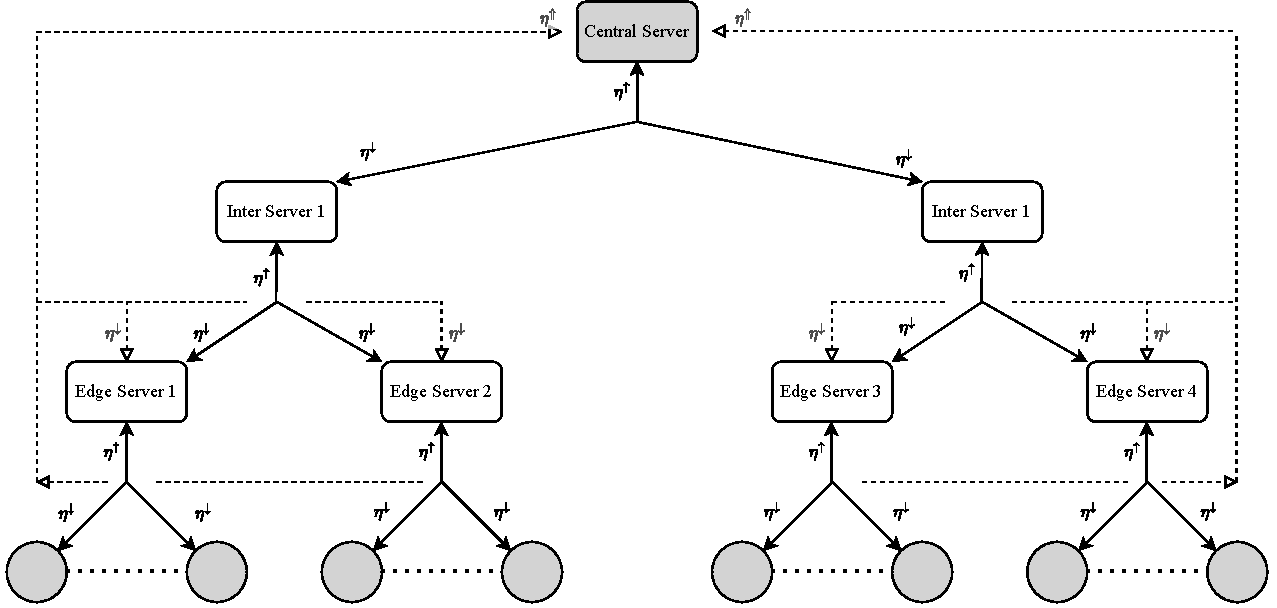
\includegraphics[clip,width=\columnwidth]{plots/Tree_Structure.drawio.pdf}
    \caption[System Diagram]{Diagram of an example B-HFL system. Solid lines represent communication links, while dashed lines represent conceptual ``residual'' connections using the underlying links. Nodes capable of training, such as clients or the central server with a proxy dataset, are in grey. When model parameters propagate up, nodes merge the incoming pseudo-gradients and update their model using the leaf-to-root learning rate $\eta^\uparrow$. The same happens when parameters flow from parents to children nodes with learning rate $\eta^\downarrow$. Since the dashed lines communicate $0$ to $K$ models, $\eta^\Uparrow$ may represent $0$ to $K$ aggregations using a $\eta^\downarrow$ learning rate.}\label{fig:TreeStructure}
\end{figure}

An example of a B-HFL system, which would be the primary deliverable of this proposal, may be seen in \cref{fig:TreeStructure}. The central server controls a proxy dataset used to train after it performs aggregation. Intermediary servers perform only aggregation. All servers send their updates to the parent after every round.

Each node, including the clients, runs at-least two stateful FedOPT server optimizers with separate learning rates, one for the leaf-to-root aggregation with the averaged pseudo-gradient $\Delta_t$ and one for parent aggregation. Even if the same leaf-to-root learning rate $\eta^\uparrow$ and root-to-leaf learning rate $\eta^\downarrow$ were to be used for all nodes in the tree or at a given level, the independent server optimiser states would distinguish the aggregation procedure of their node based on historical trends.

The residual connections serve different functions between the leaf-to-root and root-to-leaf stages. For the upward stage, they collect the client update with the highest absolute value from all edge servers, thus sending one additional model to the central server for each edge-server. The central server may then maintain independent optimiser states for each incoming ``residual'' connection. For the downward stage, they provide the edge servers with a chance to directly benefit from the training of the central server without having to rely on the models of the intermediary servers. While this last component is somewhat superfluous in the small hierarchy shown by \cref{fig:TreeStructure}, it would prove highly relevant for profound structures. For example, for deep hierarchies, parameters that receive extra training at the central server might get averaged several times before reaching the edge servers and thus influencing the leaves.



